\documentclass[parskip=full, numbers=noenddot]{scrreprt}

% language
\usepackage[english]{babel}
\usepackage[utf8]{inputenc}
\usepackage{csquotes}
\usepackage{url}
\usepackage[version=4]{mhchem}
\usepackage{siunitx}
\DeclareSIUnit\molar{\mole\per\cubic\deci\metre}
\DeclareSIUnit\Molar{\textsc{m}}
\DeclareSIUnit\calorie{cal}

% citations
\usepackage[
  natbib=true,
  backend=biber,
  doi=false,
  isbn=false,
  url=false,
  date=year,
  style=alphabetic,
  citestyle=authoryear]{biblatex}
\addbibresource{dissertation.bib}
\usepackage{varioref}

% floats
\usepackage{graphicx}
  \graphicspath{ {./graphics/} }
\usepackage{subcaption}
\usepackage{tabularx}
  \newcolumntype{L}{>{\raggedright\arraybackslash}X}
\usepackage{booktabs}
\usepackage{pgfplotstable}

\title{Quantifying the bias in SELEX procedure}
\author{Candidate number XXXXX}

\begin{document}

\maketitle
% Will deal with the intricacies of the cover pages at the very end.

\begin{abstract}
 
Summary.
 
\end{abstract}

\tableofcontents

\chapter*{List of Abbreviations}
\label{ch:abbrev}

List of Abbreviations.

\chapter{EMSA-SELEX}
\label{ch:emsaselex}

\section{Introduction}
\label{sec:emsaselex_intro}

\subsection{Physiological importance of the nucleosome, nucleosome occupancy, and gene expression}
\label{ssec:emsaselex_intro_importance}

Eukaryotes package their DNA into chromatin through a series of coiling steps.  The fundamental repeating unit of chromatin is the nucleosome.  The nucleosome consists of a histone octamer with 147 base pairs (bp) of DNA wrapped around it.

Nucleosome positioning defines where nucleosomes are positioned within the genome \citep{struhl_determinants_2013}.  In contrast, nucleosome occupancy refers to the proportion of cells in a population that have a histone at a specific region in the genome. Nucleosome positioning and nucleosome occupancy are important determinants in gene expression because nucleosomes inhibit binding of DNA-binding proteins to DNA.  Specifically, nucleosome positioning inhibits transcription by preventing RNA polymerase from accessing chromatin, and prevent binding of transcription factors to regulatory elements.  In epigenetics, histone acetylation and methylation modulate the degree of packing of chromatin, and therefore affect acessibility of DNA-binding proteins to chromatin.

\subsection{Nucleosome sequence preferences}
\label{ssec:emsaselex_intro_seqpref}

For a given 147-bp DNA sequence, the affinity of the histone octamer can vary over more than three orders of magnitude.  This is because the nucleotide sequence and the methylation state of nucleotides affect the physical flexibility of DNA, which is required for the wrapping of DNA around histone octamers.

The dinucleotide sequences AA, AT, and TA confer high flexbility to DNA.  Therefore, they are situated on the face of the helical repeat that directly interacts with the histone octamer, with a periodicity of approximately 10 bp \citep{struhl_determinants_2013}.  GC dinucleotides also occur periodically, but out of phase with the aforementioned dinucleotides.  These preferences were confirmed by a yeast-based genome-wide assay, which identified DNA regions stably wrapped in nucleosomes, and the associated dinucleotide probability distributions contributed to a computational model that confirmed these preferences \citep{segal_genomic_2006}.  Experiments with synthetic DNA in SELEX (systematic evolution of ligands by exponential enrichment) \citep{lowary_new_1998} have elucidated more rules for nucleosome positioning.  The `pentameric TG' sequence -- [(A or T)3NN(G or C)3NN]n -- has a very high affinity for the histone octamer, consistent with how AT-rich and GC-rich units confer flexibility of DNA.  `Phased TATA' sequences possessing multiple phased CTA trinucleotides also exhibit high affinity.

In contrast, the homopolymeric sequences poly(dA:dT) and poly(dG:dC) confer stiff structures that inhibit nucleosome formation.  These sequences are enriched in linker DNA between nucelosomes.  Poly(dA:dT) sequences are enriched in promoters, in particular that of \emph{Saccharomyces cerevisiae} \citep{struhl_determinants_2013}.  Depletion of nucleosomes at promoters on artificial chromosomes based on \emph{S. cerevisiae} genomic regions was shown to be dependent on the number and length of poly(dA:dT) sequences \citep{hughes_functional_2012}.

Additonally, DNA methylation disfavours nucleosome positioning \emph{in vivo}, as it increases the rigidity of DNA \citep{huff_dnmt1-independent_2014}.  Specifically, multiple tracts of methylated CpG sequences islands makes DNA have lower rise and twist along with higher roll values, thus making the DNA stiffer \citep{rao_systematic_2018, perez_impact_2012}.  However, the negative correlation between nucleosome occupancy and DNA methylation varies according to the genomic location.  For example, this negative correlation holds for CTCF regions, but not at promoters \citep{kelly_genome-wide_2012}.

\subsection{Purpose of study}
\label{ssec:emsaselex_intro_why}

% Start with research questions/unknowns:
%   1. A clean in vitro investigation of sequence preference for CpG methylation is not available.
%   2. No-one has explored all-mC ligand preference.  This is important because CH methylation has physiological roles...

To date, clean \emph{in vitro} sequence preference data for CpG methylation is not available.  This is in contrast to sequence preference data derived from MNase-seq on existing genomes in previous studies \citep{struhl_determinants_2013, segal_genomic_2006, huff_dnmt1-independent_2014}.  Furthermore, there has been no exploration into the effects of CH methylation (non-CpG methylation) on sequence preferences of nucleosomes.  Although CpG methylation is the predominant chemical modification of eukaryotic DNA, playing roles in gene regulation and physiology, CH methylation regulates development of stem cells and neurons \citep{guo_distribution_2014}.

SELEX is a promising method to identify the DNA sequences preferred for nucleosome positioning.  Unlike MNase-seq, SELEX employs a random DNA library, which has a higher complexity than genomic sequences and a more homogenous background sequence distribution.  \citet{lowary_new_1998} employed SELEX in uncovering sequence-based rules for nucleosome positioning, but analysis was limited by the technology at the time.  This project extended on their study by employing sequencing to a higher depth, allowing identification of signals with higher information content.

In this project, I aimed to study the sequence specificity of the nucleosome on methylated and non-methylated DNA.  I conducted four cycles of nucleosome SELEX using random DNA as the initial input library.  In each cycle, I reconstituted nucleosomes from \emph{Xenopus laevis} histone octamer and 147-bp DNA \citep{dyer_reconstitution_2003} methylated at various levels.  This included CpG methylation, methylation at all cytosines, and methylation at half the cytosines.  I extracted the DNA bound to nucleosomes at each cycle for sequencing, then assessed the distribution of mononucleotides and dinucleotides using Fourier transform \citep{lowary_new_1998, zhu_interaction_2018}.  Subsequently, I investigated the effect of histone octamer binding on the enrichment of mononucleotides in the sequencing libraries by producing 9-mer plots.

\section{Materials and Methods}
\label{sec:emsaselex_methods}

\subsection{DNA ligand design and preparation}
\label{ssec:emsaselex_methods_lig}

The sequence of the initial input library is 5$'$ GCTCTTCCGATCT nnnnnnnnnnnnnnnnnnnn AGATCGGAAGAGC 3$'$, where n denotes any nucleotide chosen at random. The input library DNA was made to 200 \SI{200}{\nano\Molar} in TE buffer with \SI{0.2}{\milli\Molar} EDTA.

PCR amplification was adapted from manufacturer's recommended protocols for Phusion High-Fidelity DNA Polymerase (ThermoFisher, cat no F530).  The sequence of the forward primer was 5$'$ CCCTACACGAC GCTCTTCC 3$'$, and the sequence of the reverse primer was 3$'$ GCCTTCTCG TGTGCAGAC 5$'$.  Thirteen cycles of PCR with recommended temperatures were followed by ten cycles with the \SI{98}{\celsius} denaturation temperature replaced with \SI{72}{\celsius}.  For the `half-C-methylated group', half of the dCTPs were replaced with 5-methylcytosine, and for the `all-C-methylated group', all of the dCTPs were replaced with 5-methylcytosine.   For CpG-methylation, methyltransferase (M.SssI) was added to DNA in conjunction with S-adenosylmethionine and \ce{MgCl2}, then incubated according to manufacturer's protocols.

\subsection{SELEX}
\label{ssec:emsaselex_methods_selex}

Nucleosome reconstitution procedures were adapted from \citet{dyer_reconstitution_2003} (`Reconstitution of Nucleosome Core Particles'), using \SI{2}{\Molar} \ce{KCl}.  Histone:DNA ratios were 1.48:1, 0.74:1, 0.37:1, 0.19:1, and 0.09:1. % is the last part necessary given that I'm likely going to put it in a figure?

To verify results, reconstituted nucleosomes were analysed by EMSA by using TBE 6\% DNA retardation gel and 0.2\% TBE buffer on ice.  Gel bands corresponding to unbound DNA and to reconstituted nucleosomes were sliced.  The sliced bands were dissolved in \SI{70}{\micro\litre} Tris pH 8.0, and then incubated at \SI{70}{\celsius} overnight.

Eluted DNA was amplified using procedures adapted from manufacturer's recommended protocols for Phusion High-Fidelity DNA Polymerase.  Here, 21 cycles of PCR with a \SI{98}{\celsius} denaturation temperature and a \SI{67}{\celsius} annealing temperature was followed by ten cycles with a \SI{79}{\celsius} denaturation temperature and a \SI{64}{\celsius} annealing temperature.

\subsection{Sequencing}
\label{ssec:emsaselex_methods_seq}

After SELEX, the eluted DNA was barcoded for sequencing.  Amplification was carried out using the procedures recommended for Phusion DNA polymerase for 29 PCR cycles, using \SI{5}{\micro\Molar} barcoded PE primer obtained from IDT.  All barcoded DNA was then pooled together and purified using 1.2x AMPure beads (Beckman Coulter) according to manufacturer's protocols.  Subsequently, the DNA was diluted to \SI{2}{\nano\Molar}.  Illumina HiSeq 4000 was then used for sequencing, following standard protocols, with $>$ 60 bp paired-end settings.  Raw sequences are demultiplexed, then the R1 and R2 reads of paired-end sequencing were merged according to \citet{zhu_interaction_2018}.

\subsection{Data analysis}
\label{ssec:emsaselex_methods_anal}

Fast Fourier transformation (FFT) was performed using the position along the sequence read as the time domain and the frequency of mononucleotides or dinucleotides at a specific position within the sequence as the frequency domain, following \citet{zhu_interaction_2018}.  From this, power spectra for mononucleotides and dinucleotides were obtained.  The phase of FFT was also examined at 0.102 per base pair.

% This can easily be trivial information and will likely be deleted.
For each library, the frequency of all possible 9-mers of nucleotide sequences were counted.  x-y scatter plots were generated to compare the counts between libraries, and the Pearson correlation coefficient was calculated for each scatter plot.

\section{Results}
\label{sec:emsaselex_results}

% replace with properly-drawn version later
\begin{figure}[htpb]
  \centering
  \includegraphics[width=\textwidth]{selexoverview}
  \caption{Overview of nucleosome EMSA-SELEX procedure}
  \label{fig:selex}
\end{figure}

Four cycles of nucleosome EMSA SELEX (figure~\ref{fig:selex}) were carried out.  147-bp oligonucleotides with a 101-bp central random sequence -- termed lig147 \citep{zhu_interaction_2018} -- constituted the initial input library.  The experiment had four groups: plain (non-methylated) DNA, CpG-methylated DNA, DNA with all cytosines methylated (all-C-methylated DNA), and DNA with half of its cytosines methylated (half-C-methylated DNA).

\subsection{Nucleosome reconstitution}
\label{ssec:reconstnuc}

EMSA in all cycles yielded one strong band between 100 and 200 bp. It also yielded bands corresponding to reconstituted nucleosomes that became fainter as the proportion of histone octamer decreased in the solution (figure~\ref{fig:reconstnuc}).  DNA ligands that were not bound to nucleosomes and ligands that were bound to nucleosomes were eluted and then sequenced.

% add ticks for weights on gels
% put the ratios onto the images instead of in the caption
\begin{figure}[htpb]
  \centering
  \begin{subfigure}[htpb]{0.4\textwidth}
    \centering
    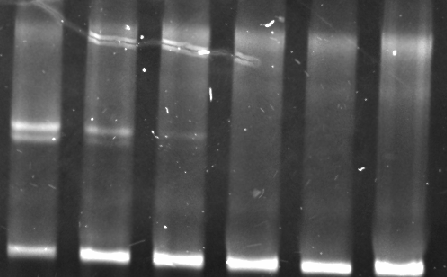
\includegraphics[width=\textwidth]{reconstnuc_a}
    \caption{Plain DNA}
    \label{fig:reconstnuc_a}
  \end{subfigure}
  \begin{subfigure}[htpb]{0.4\textwidth}
    \centering
    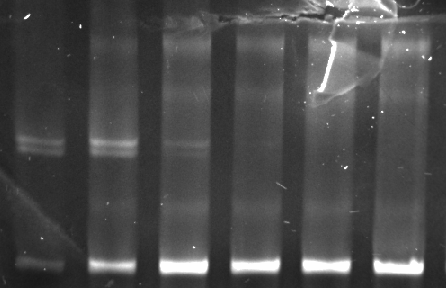
\includegraphics[width=\textwidth]{reconstnuc_b}
    \caption{Half-C-methylated DNA}
    \label{fig:reconstnuc_b}
  \end{subfigure}
  \begin{subfigure}[htpb]{0.4\textwidth}
    \centering
    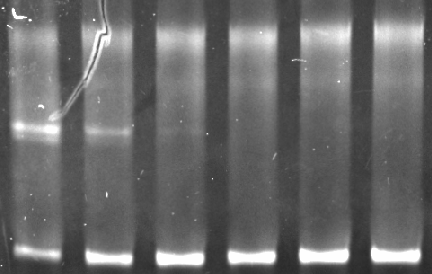
\includegraphics[width=\textwidth]{reconstnuc_c}
    \caption{All-C-methylated DNA}
    \label{fig:reconstnuc_c}
  \end{subfigure}
  \begin{subfigure}[htpb]{0.4\textwidth}
    \centering
    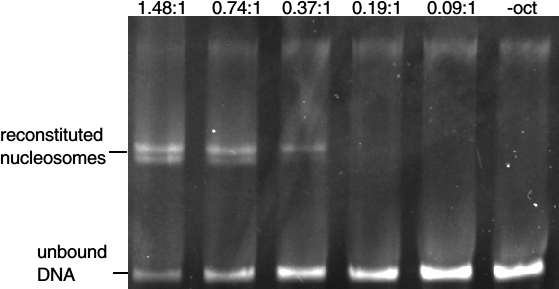
\includegraphics[width=\textwidth]{reconstnuc_d}
    \caption{CpG-methylated DNA}
    \label{fig:reconstnuc_d}
  \end{subfigure}
  \caption{First-cycle EMSA in 6\% DNA retardation gels for the four experimental groups.  Lanes for all images correspond to these histone:octamer ratios (left to right): (1) 1.48:1, (2) 0.74:1, (3) 0.37:1, (4) 0.19:1, (5) 0.09:1, and (6) DNA without histone octamer added.  These results are representative for all cycles.}
  \label{fig:reconstnuc}
\end{figure}

The frequency of all mononucleotide and dinucleotide sequences at each position along the reads were calculated (figure~\ref{fig:freqplots}).  The data from the fourth cycle of EMSA-SELEX were used in all subsequent analyses because they exhibited the strongest signals.  All DNA libraries bound to nucleosomes showed a clear periodicity in mononucleotide and dinucleotide frequencies, but the periodicity in the plain DNA libraries was less clear.

\begin{figure}[htpb]
  \centering
  \begin{subfigure}[htpb]{0.5\textwidth}
    \centering
    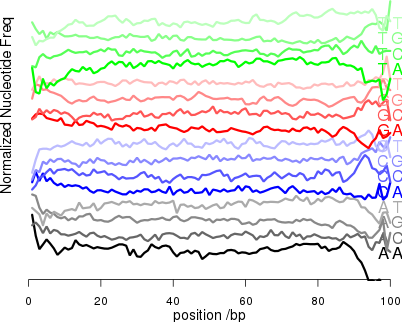
\includegraphics[width=0.5\textwidth]{emsa_e8_counts}
    \caption{Plain DNA}
    \label{fig:freqplots_e8}
  \end{subfigure}
  \begin{subfigure}[htpb]{0.5\textwidth}
    \centering
    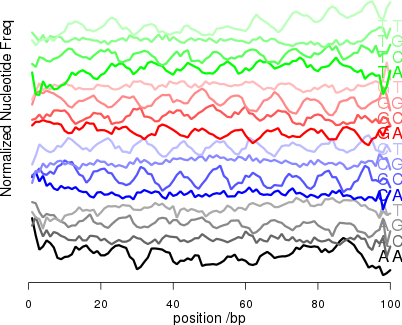
\includegraphics[width=0.5\textwidth]{emsa_f8_counts}
    \caption{Half-C-methylated}
    \label{fig:freqplots_f8}
  \end{subfigure}
  \begin{subfigure}[htpb]{0.5\textwidth}
    \centering
    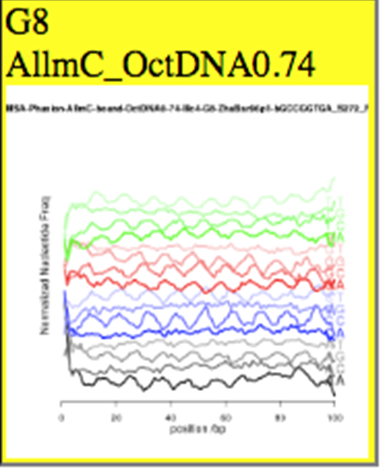
\includegraphics[width=0.5\textwidth]{emsa_g8_counts}
    \caption{All-C-methylated}
    \label{fig:freqplots_g8}
  \end{subfigure}
  \begin{subfigure}[htpb]{0.5\textwidth}
    \centering
    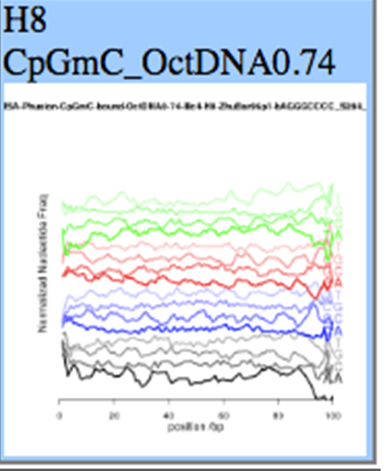
\includegraphics[width=0.5\textwidth]{emsa_h8_counts}
    \caption{CpG methylated}
    \label{fig:freqplots_h8}
  \end{subfigure}
  \caption{Frequencies of each mononucleotide and dinucleotide along the sequencing reads from libraries corresponding to 1:0.74 octamer:DNA ratios for the fourth cycle of EMSA-SELEX}
  \label{fig:freqplots}
\end{figure}

An additional library of plain DNA bound to nucleosomes prepared with additional rounds of AMPure bead purification to enrich the signals was analysed.  Characterisation of frequencies of mononucleotides at each position along the reads for this library yielded clear periodicities (figure~\ref{fig:enriched_counts}), which were confirmed to be approximately 10 bp by fast Fourier transform (figure~\ref{fig:enriched_power}).  However, this library exhibited biases towards G and T nucleotides.

\begin{figure}[htpb]
  \centering
  \begin{subfigure}[htpb]{\textwidth}
    \centering
    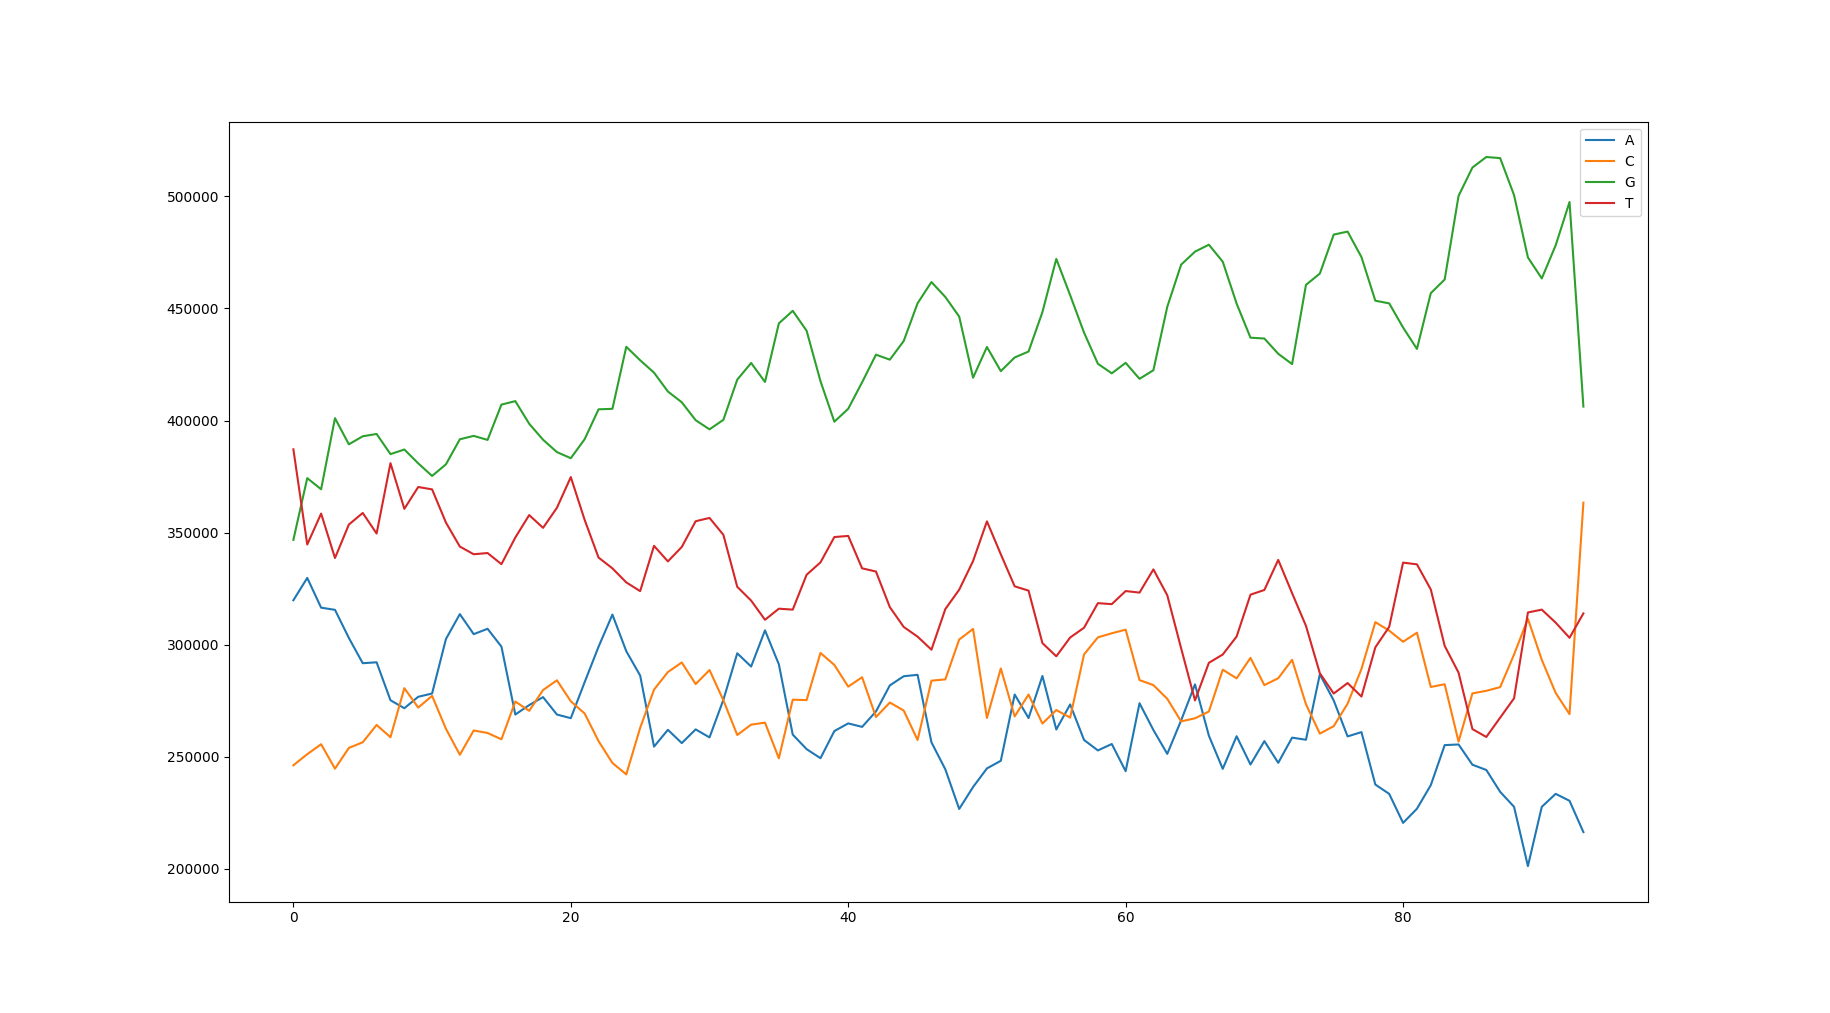
\includegraphics[width=\textwidth]{enriched-counts}
    \caption{}
    \label{fig:enriched_counts}
  \end{subfigure}
  \begin{subfigure}[htpb]{\textwidth}
    \centering
    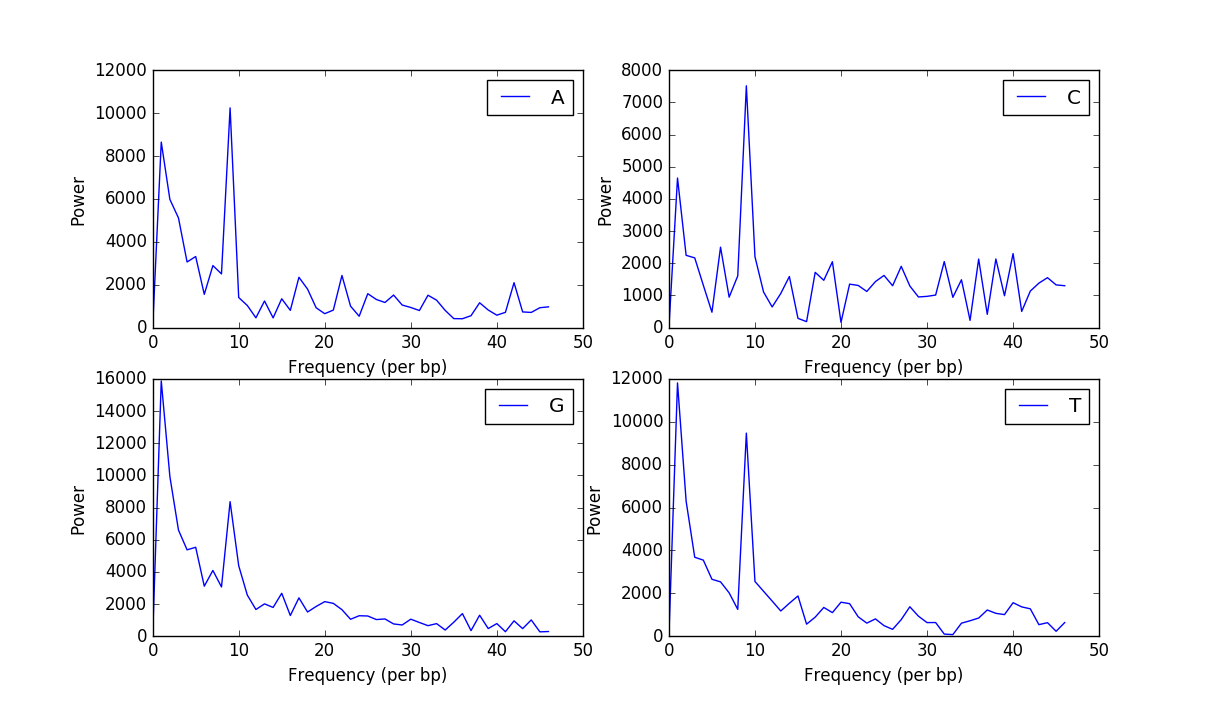
\includegraphics[width=\textwidth]{enriched-power}
    \caption{}
    \label{fig:enriched_power}
  \end{subfigure}
  \caption{Analysis of a library of plain DNA bound to nucleosomes enriched for signal. (a) shows the nucleotide counts as a function of position along the reads, and (b) shows the fast Fourier transform power spectra for the four nucleotides.}
  \label{fig:enriched}
\end{figure}

In contrast, all DNA libraries not bound to nucleosomes were depleted of this periodic signal.  This periodicity was assessed by fast Fourier transform, and the resulting power spectra showed that the periodicity was near 10 bp (figure~\ref{fig:powerspectra}).  Specifically, half-C-methylated and all-C-methylated DNA showed the strongest signals, % QUESTION: quantification of strength/height of peak?
CpG-methylated DNA showed signals of intermediate strength, and plain DNA showed the weakest signals.  Among the octamer-to-DNA concentrations tested, the 1:0.74 ratio gave rise to the strongest signals, and the signal intensity decreased as the proportion of DNA increased (data not shown).  Libraries corresponding to this octamer:DNA ratio were therefore used for all subsequent analyses.

% kind of a placeholder at the moment...
\begin{figure}[htpb]
  \centering
  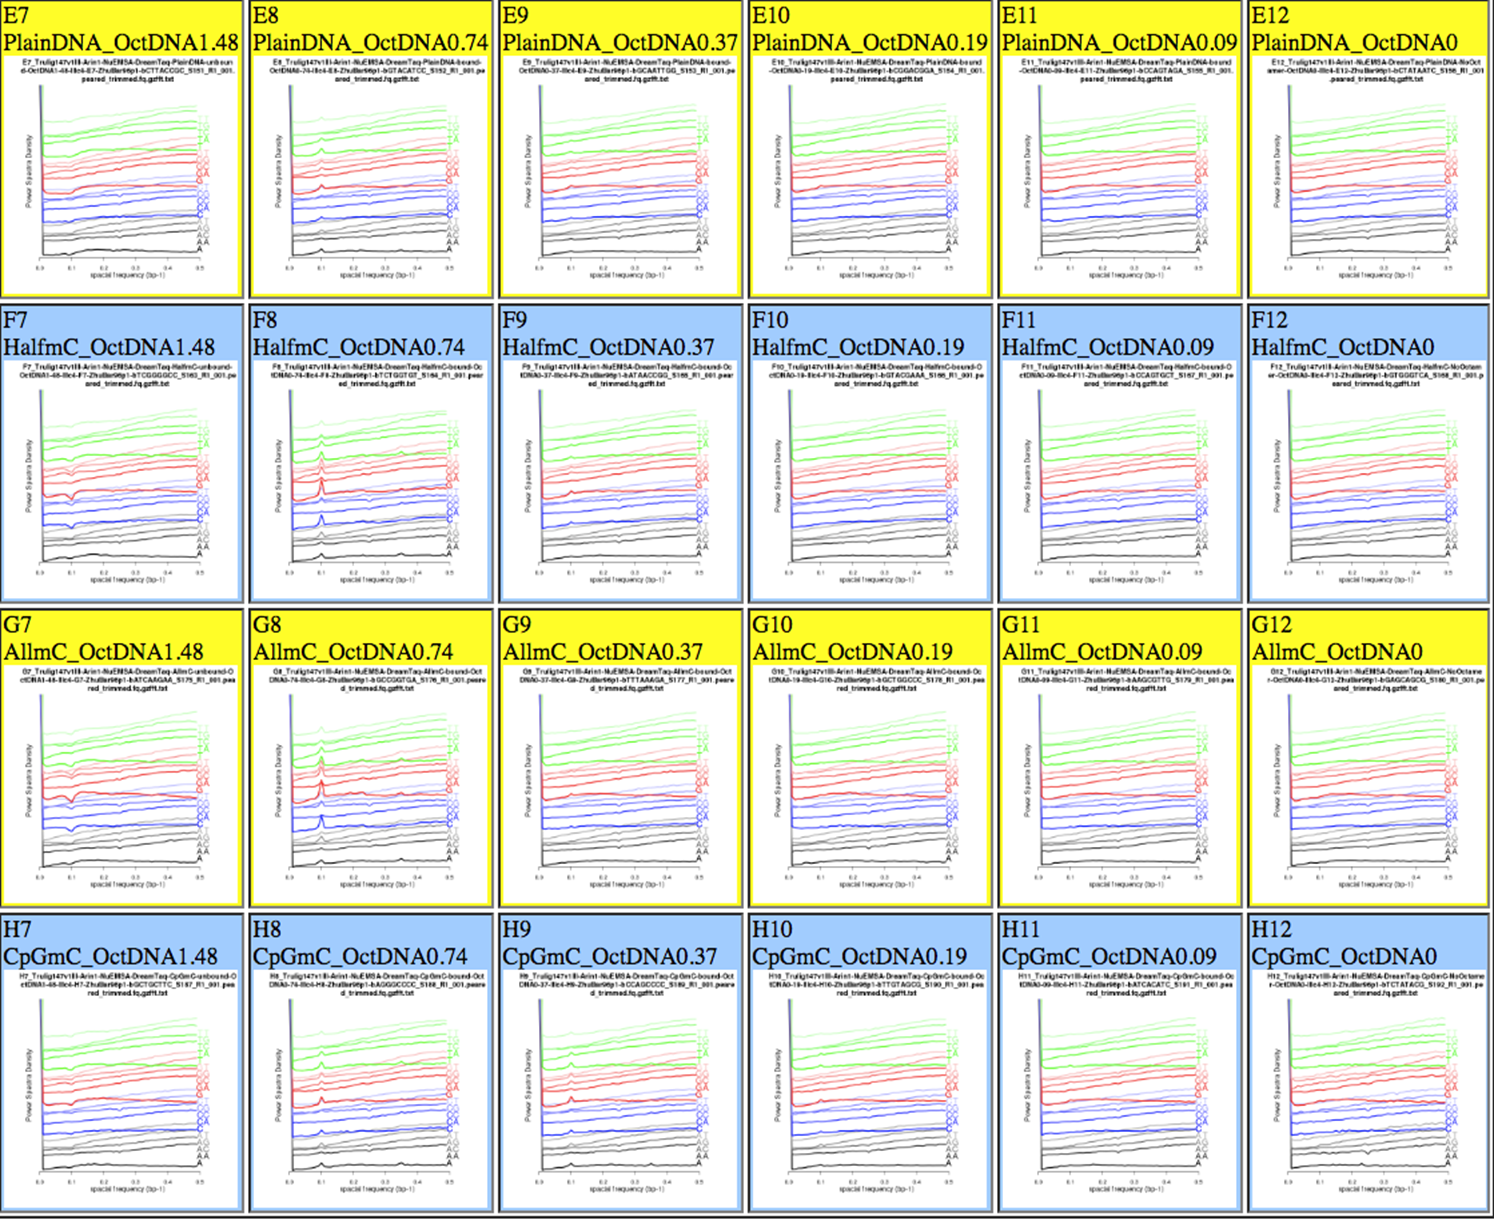
\includegraphics[width=\textwidth]{emsacycle4all}
  \caption{Power spectra derived from the frequencies of all mononucleotide and dinucleotides.  Libraries are from the fourth cycle of EMSA-SELEX.  The ligand type and the octamer:DNA ratios were varied.}
  \label{fig:powerspectra}
\end{figure}

\subsection{Sequence preferences from fast Fourier transform analysis}
\label{ssec:nuseqpref_fft}
% ORIGINAL PLAN:
%% - The sequence preferences of nucleosome 
%% - Disfavored sequences of nucleosome
%% - Methylation effects on nucleosome’s sequence preference

The phases and the amplitudes resulting from the fast Fourier transforms were then characterised, based on a frequency of 10.2 bp (figure~\ref{fig:radial_mc}).

When the cytosines were methylated, the amplitude for dinucleotides beginning with C increased, and their phases became more aligned.  Specifically, in the plain DNA library, the CA, CC, CG, and CT sequences were spread out over phases of \ang{80} to \ang{260} (figure~\ref{fig:radial_mc_plain}).  In the half-C-methylated and all-C-methylated libraries for the same octamer:DNA ratio, these sequences were spead out over phases of \ang{70} to \ang{140} (figures~\ref{fig:radial_mc_halfmc} and~\ref{fig:radial_mc_allmc}).  These dinucleotides became more aligned to TC.  The phases of the reverse complements of these dinucleotides -- namely GA, GC, and GG -- also became more aligned when the cytosines are methylated.   Using the AA sequence as a reference, the amplitudes for CT and CA were greater in the all-C-methylated library than in the half-C-methylated library, but the amplitude for CG slightly reduced.
% QUESTION: is there a better way to describe the `spread' of the CX sequences to replace eyeballing and saying `yeah, it looks like they're less spread alright'.

These effects were less pronounced for CpG methylation (figure~\ref{fig:radial_mc_cpg}). % topic sentence
Using the AA sequence as a reference, the amplitudes of CC and CT increased.  Similar to the other experimental groups, the amplitude of CG exhibited a slight decrease.  However, the CA, CC, CG, and CT sequences were still spread over a wide range of phases, covering \ang{80} to \ang{160}.

\begin{figure}[htpb]
  \centering
  \begin{subfigure}[htpb]{0.5\textwidth}
    \centering
    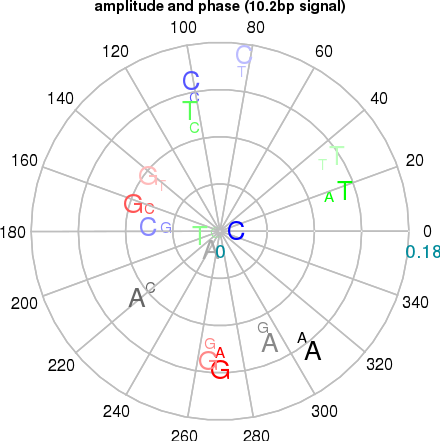
\includegraphics[width=0.5\textwidth]{emsa_e8_radial}
    \caption{Plain DNA}
    \label{fig:radial_mc_plain}
  \end{subfigure}
  \begin{subfigure}[htpb]{0.5\textwidth}
    \centering
    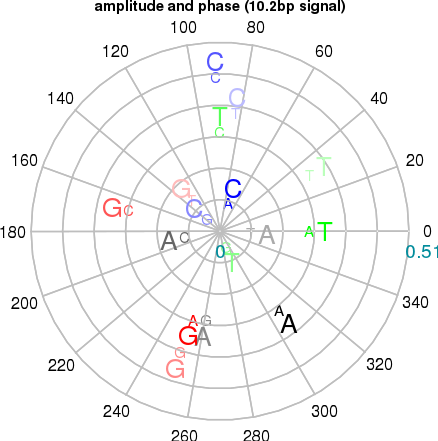
\includegraphics[width=0.5\textwidth]{emsa_f8_radial}
    \caption{Half-C-methylated}
    \label{fig:radial_mc_halfmc}
  \end{subfigure}
  \begin{subfigure}[htpb]{0.5\textwidth}
    \centering
    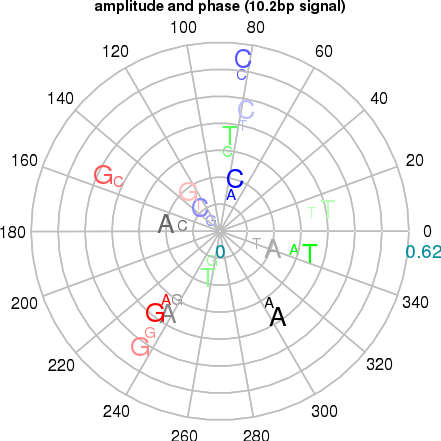
\includegraphics[width=0.5\textwidth]{emsa_g8_radial}
    \caption{All-C-methylated}
    \label{fig:radial_mc_allmc}
  \end{subfigure}
  \begin{subfigure}[htpb]{0.5\textwidth}
    \centering
    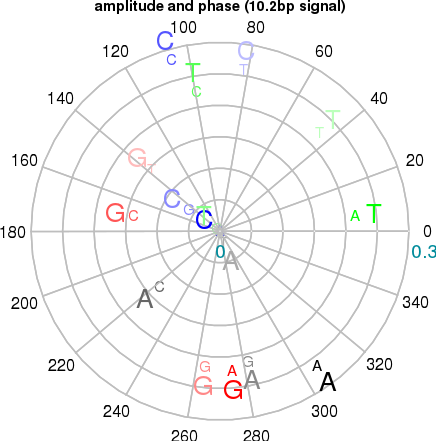
\includegraphics[width=0.5\textwidth]{emsa_h8_radial}
    \caption{CpG methylated}
    \label{fig:radial_mc_cpg}
  \end{subfigure}
  \caption{Effects of cytosine methylation: radial plots showing amplitudes and phases for each dinucleotide}
  \label{fig:radial_mc}
\end{figure}

% could discuss why some things are enriched and some are depleted, but the effect size isn't great as they're all around 1 (which is sort of expected as histone octamers only bind loosely to DNA).  Theoretically to evaluate how significant the deviations from 1 are we would have to make at least three replicates, but we didn't (they're bloody expensive too) -- can also put this in the discussion
Certain dinucleotides containing cytosines were enriched when the cytosines were methylated, especially in CpG methylation (figure~\ref{fig:c2nt}).  In particular CC, CG, and GC were enriched in the CpG methylated group.  In constrast, CC was depleted in the all-C-methylated group.  However, in all samples, deviations from a 1:1 ratio were small.

% Use R to replace this with a dot plot later
\begin{figure}[htpb]
  \centering
  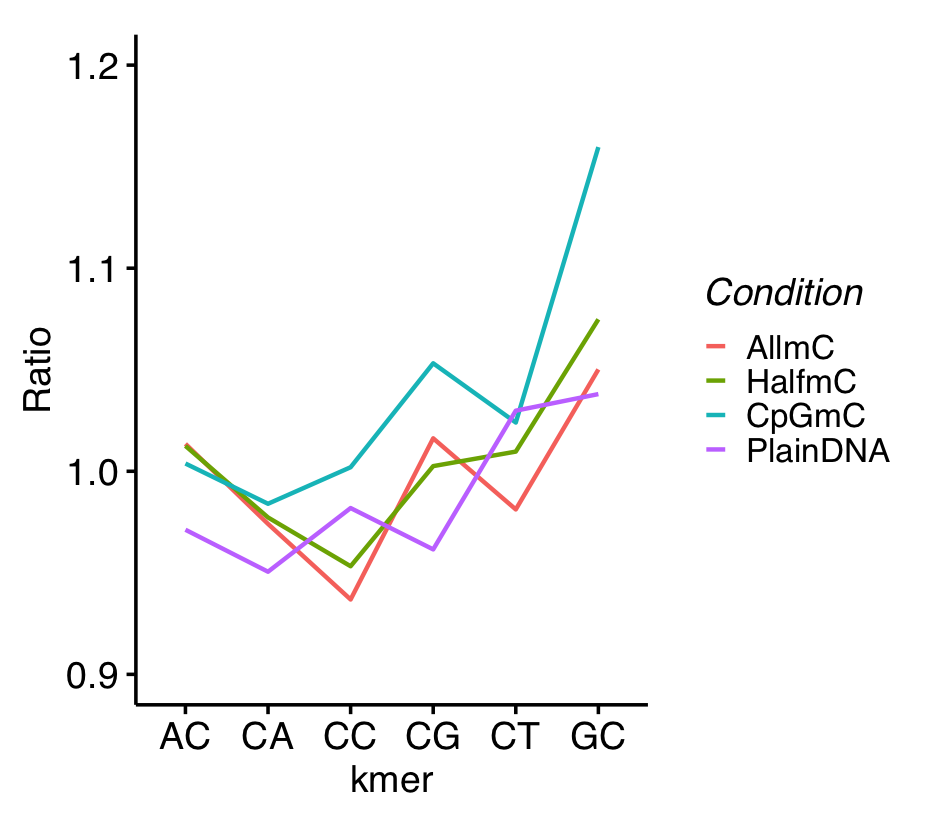
\includegraphics[width=\textwidth]{c2nt}
  \caption{Enrichment of dinucleotides in the 0.74:1 octamer:DNA ratio libraries for each experimental group.  The number of occurences of each dinucleotide in each library was calculated.  Dividing the count from the bound DNA library by the count from the unbound DNA library gave the ratios shown.} 
  \label{fig:c2nt}
\end{figure}

\subsection{Sequence preferences from sequence \emph{k}-mer counts}
\label{ssec:nuseqpref_kmer}

For each library, the frequency of each possible continuous 9-mer of nucleotides was counted.  With the half-C-methylated, all-C-methylated, and CpG-methylated experimental groups (figure~\ref{fig:kmer_bound}), the unbound libraries were enriched in A and T compared to the bound libraries.  This effect was less significant when all cytosines were methylated (figure~\ref{fig:kmer_bound_all}).  However, both the bound and unbound all-C-methylated libraries were enriched in A and T as compared to the corresponding plain DNA libraries (figure~\ref{fig:kmer_bias}). % interpretation in discussion

\begin{figure}[htpb]
  \centering
  \begin{subfigure}[htpb]{0.7\textwidth}
    \centering
    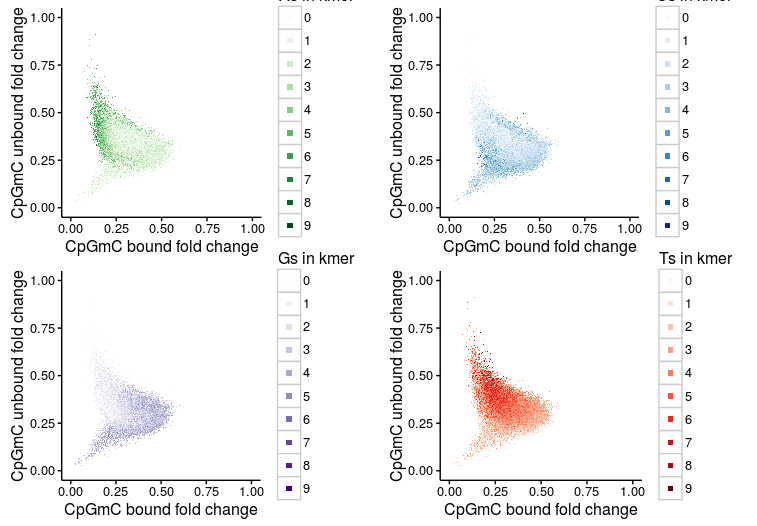
\includegraphics[width=0.7\textwidth]{kmer_CpGubXCpGb}
    \caption{CpG methylated}
    \label{fig:kmer_bound_cpg}
  \end{subfigure}
  \begin{subfigure}[htpb]{0.7\textwidth}
    \centering
    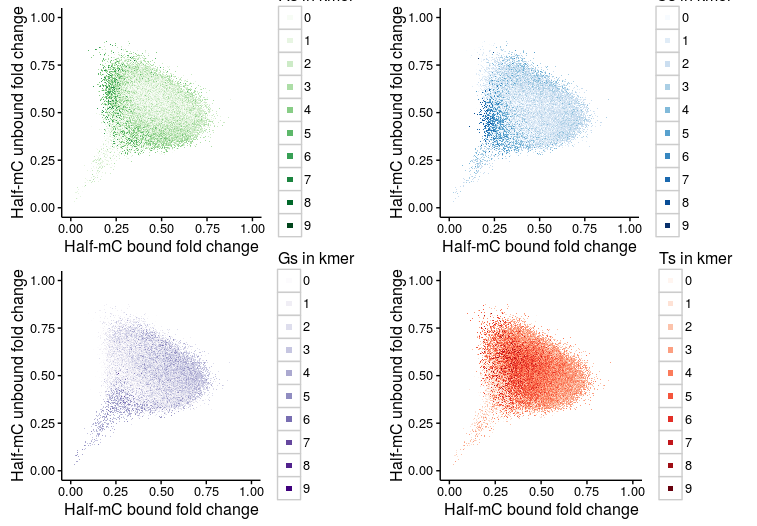
\includegraphics[width=0.7\textwidth]{kmer_halfubXhalfb}
    \caption{Half-C-methylated}
    \label{fig:kmer_bound_half}
  \end{subfigure}
  \begin{subfigure}[htpb]{0.7\textwidth}
    \centering
    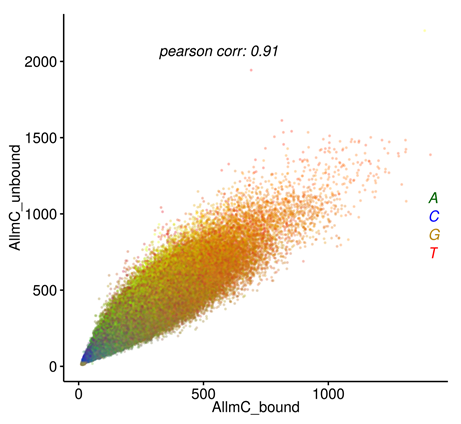
\includegraphics[width=0.7\textwidth]{kmer_allubXallb}
    \caption{All-C-methylated}
    \label{fig:kmer_bound_all}
  \end{subfigure}
  \caption{9-mer count scatter plots showing the effect of nucleosome reconstitution on each experimental group.  Horizontal axes correspond to DNA bound in nucleosomes, while vertical axes correspond to unbound DNA.  Green indicates 9-mers consisting of predominantly adenines, blue cytosines, yellow guanines, and red thymines.  Data for plain DNA not shown as signal was too weak.}
  \label{fig:kmer_bound}
\end{figure}

\begin{figure}[htpb]
  \centering
  \begin{subfigure}[htpb]{0.7\textwidth}
    \centering
    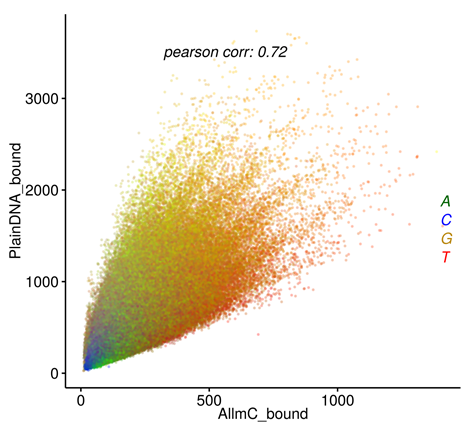
\includegraphics[width=0.7\textwidth]{kmer_plainbXallb}
    \caption{Bound DNA}
    \label{fig:kmer_bias_bound}
  \end{subfigure}
  \begin{subfigure}[htpb]{0.7\textwidth}
    \centering
    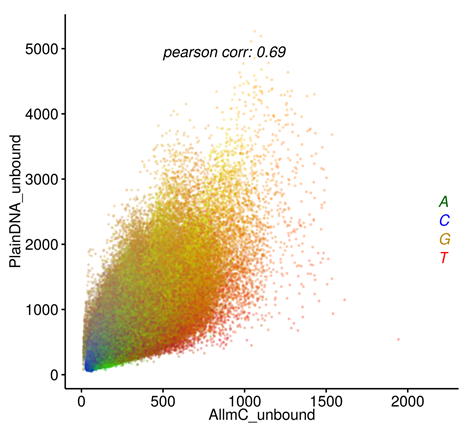
\includegraphics[width=0.7\textwidth]{kmer_plainubXallub}
    \caption{Unbound DNA}
    \label{fig:kmer_bias_unbound}
  \end{subfigure}
  \caption{9-mer count scatter plots showing sequence biases.  Horizontal axes correspond to the all-C-methylated libraries, while vertical axes correspond to the plain DNA libraries.  Green indicates 9-mers consisting of predominantly adenines, blue cytosines, yellow guanines, and red thymines.}
  \label{fig:kmer_bias}
\end{figure}

The frequency of continuous stretches of adenines (A-stretches) were also counted in each library (figure~\ref{fig:astretch}).  Methylation was associated with A-stretches being less represented in the libraries containing DNA bound to nucleosomes.  Compared to plain DNA, the half-C-methylated and all-C-methylated groups exhibited greater depletions in A-stretches.  This effect was more pronounced in the CpG methylated group.

% make this look more glamorous later by changing around the R code.  it's already informative
\begin{figure}[htpb]
  \centering
  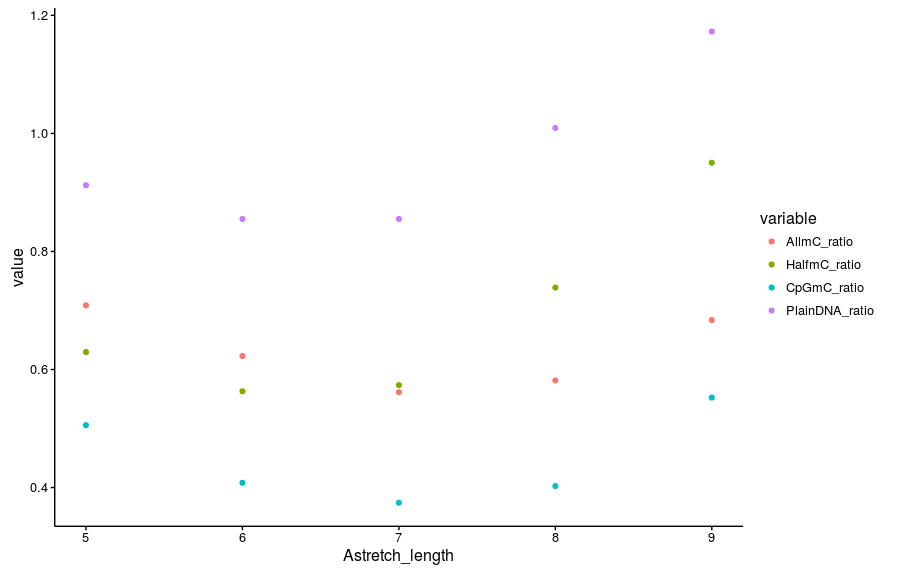
\includegraphics[width=\textwidth]{astretch}
  \caption{Enrichment of continuous stretches of adenines for each experimental group.  The number of occurences of each k-mer of adenine stretches in each library was calculated (e.g. `5' corresponds to `AAAAA').  Dividing the count from the bound DNA library by the count from the unbound DNA library gave the ratios shown.}
  \label{fig:astretch}
\end{figure}

\section{Discussion}
\label{sec:emsaselex_discussion}

%%% GUIDELINES FROM DEPARTMENT
% brief recapitulation of major conclusions and evidence that supports them
% discuss how results relate to previously published work, and to the ideas and models currently favoured in the field
% suggestions as to how experiments might be improved and refined
% explain what further work you would have done if you had had more time

% is this first point absolutely necessary?
From nucleosome EMSA-SELEX, nucleosome binding introduces an approximately 10-bp periodicity in mononucleotide and dinucleotide frequencies, confirming previous studies that suggest a $\sim$10-bp helical repeat and positioning of bendable dinucleotides at the same periodicity \citep{struhl_determinants_2013}.  The absence of nucleosome binding is associated with a depletion of this periodic signal.  Furthermore, phases and amplitudes of the relevant dinucleotides supported previous findings that indicate the TA dinucleotide occurs at this periodicity and out of phase with GC.  This was supported by the relatively high amplitudes of these nucleotides.  However, in the plain DNA group (figure~\ref{fig:radial_mc_plain}) TA (\ang{20}) did not seem to occur completely out of phase with GC (\ang{150}), but this is likely because the periodicity in this group was not as strong as the groups with methylated DNA (figure~\ref{fig:freqplots_e8}).  % Analysing the plain DNA library enriched for signal could confirm TA and GC periodicities.
% link this to physiological relevance of these preferences

When cytosines were methylated, the amplitudes of CC, GG, and GC dinucleotides increased, and the phases of CC, CT, TC, and CA along with that of their reverse complements lined up more.  The effect is strongest for the all-C-methylated group, followed by the half-C-methylated and CpG methylated groups.  Methylation of cytosines makes DNA more rigid \citep{rao_systematic_2018, perez_impact_2012}, so a possible explanation of this observation is that rigid sequences are more strongly associated with the phase corresponding to linker DNA as more cytosines are methylated.  Another explanation for the phase changes is that methylated cytosines are structurally similar to thymines and therefore behaves more like thymines on account of the base becoming more bulky.  This explains TC and CC having similar phases, but does not explain why TT does not share this similarity.  It should also be noted that the amplitude of CG exhibited a small decrease in the all-C-methylated and CpG methylated groups, the two groups in which all CG sequences are methylated at the cytosine.  % QUESTION: why?? what is the significance of this??
% link this to physiological relevance of methylation

From the \emph{k}-mer plots, libraries from unbound DNA were enriched in A and T compared to bound DNA, but this effect was less pronounced when all cytosines were methylated.  Investigating sequence enrichments in the all-C-methylated group relative to the plain DNA group revealed that the same bias towards A and T was present in both unbound and bound DNA, pointing the reason for this bias towards PCR.  This conclusion is supported by how most DNA polymerases have difficulty incorporating methylated cytosines in PCR (Yin, personal communication). % replace with a better citation if I can find one; QUESTION: evidence that DNA polymerases don't like to incorporate methylated cytosines in PCR
Development of a model to quantify the biases introduced by methylated cytosines in the PCR reaction mixture would aid in determining whether cytosine methylation leads to enrichment of particular nucleotides in nucleosome reconstitution.  The linear model developed to explain the contribution of enzyme and dNTP sources to PCR bias (table~\ref{tab:linearmodel_coeffs}) suggested that among the dNTP sources tested, dNTPs from Zymo Research with methylated cytosines introduced the greatest bias in PCR.  However, this bias is small, with the greatest absolute value among the coefficients at 9.4\%, and within the range of that of dNTPs from Agilent Technologies that did not contain methylated cytosines.  Extending the PCR bias experiments to cover more cycles of PCR could confirm whether methylated cytosines are the main contributor to the bias in the \emph{k}-mer plots as barcoding involves more than 24 cycles of PCR, the number of cycles investigated in the PCR bias experiments.

%% - The underlying mechanism leading to nucleosome’s sequence preference
%% - Physiological meaning of such preference
%% - Physiological relevance of the methylation effect
%% - A few discussions about Troubleshooting

% I anticipate this to be A LOT shorter

% Debugging should probably be in a separate subsection in the results or discussion section

%% After the DNA was eluted, barcodes were added using DreamTaq or Phusion (both ThermoFisher) as DNA polymerases.  Gel electrophoresis of the products amplified by DreamTaq yielded bands corresponding to 147 base pairs (figure~\ref{fig:barcoding_a}).  However, gel electrophoresis of the products amplified by Phusion using recommended protocols did not yield this band (figure~\ref{fig:barcoding_b}).

%% Repeating the Phusion amplification using qPCR yielded saturation curves (figure~\ref{fig:qpcr}), suggesting that amplification indeed took place.  As qPCR required a lower concentration of the template, it was hypothesised that Phusion initially failed because the ligand was too concentrated.  Different DNA polymerases from different vendors are efficient with differing template concentrations – for example, DreamTaq requires ... while Phusion requires ... (citation needed).  Therefore, I diluted the template DNA further by adding \SI{70}{\micro\litre} dilution buffer to each well. The resulting 8\% TBE gel yielded the band corresponding to 147 base pairs (figure~\ref{fig:barcoding_c}), confirming the hypothesis.

%% \begin{figure}[htpb]
%%   \centering
%%   \begin{subfigure}[htpb]{0.4\textwidth}
%%     \centering
%%     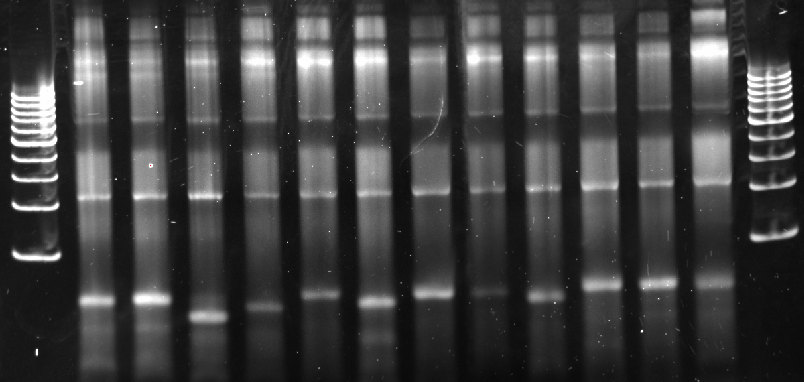
\includegraphics[width=\textwidth]{dreamtaq}
%%     \caption{A}
%%     \label{fig:barcoding_a}
%%   \end{subfigure}
%%   \begin{subfigure}[htpb]{0.4\textwidth}
%%     \centering
%%     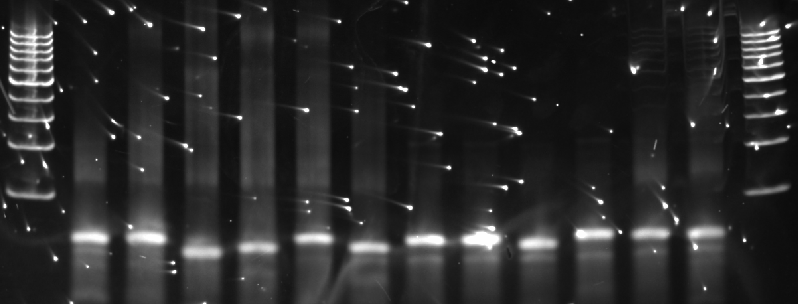
\includegraphics[width=\textwidth]{phusion_old_a}
%%     \caption{B}
%%     \label{fig:barcoding_b}
%%   \end{subfigure}
%%   \begin{subfigure}[htpb]{0.4\textwidth}
%%     \centering
%%     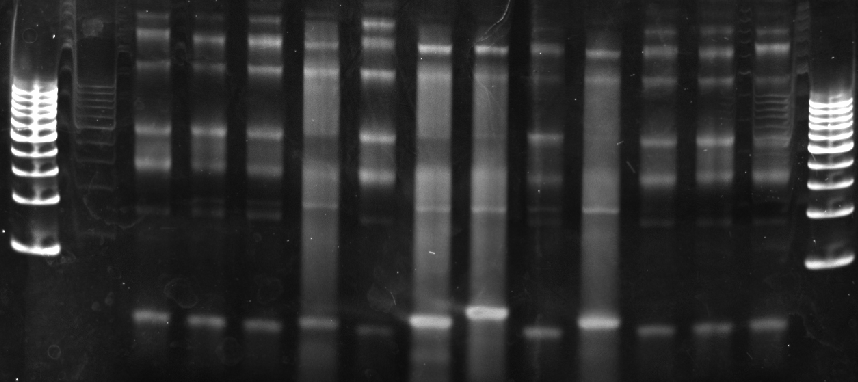
\includegraphics[width=\textwidth]{phusion_new_a}
%%     \caption{C}
%%     \label{fig:barcoding_c}
%%   \end{subfigure}
%%   \begin{subfigure}[htpb]{0.4\textwidth}
%%     \centering
%%     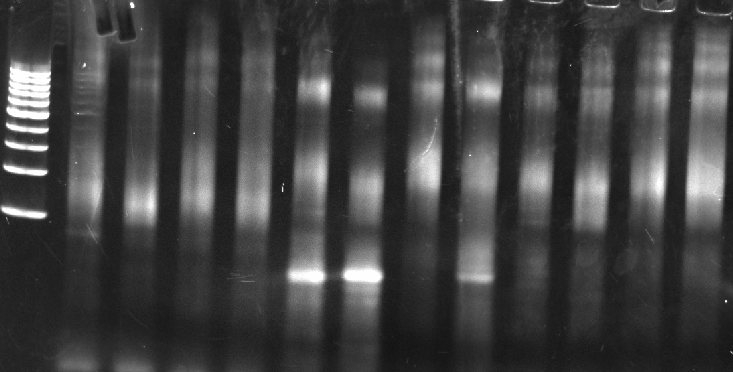
\includegraphics[width=\textwidth]{qpcrgel}
%%     \caption{D}
%%     \label{fig:barcoding_d}
%%   \end{subfigure}
%%   \caption{A - DreamTaq gel, B - old Phusion gels for rows A and B, C - new Phusion gels for rows A and B, D - qPCR gel}
%%   \label{fig:barcoding}
%% \end{figure}

%% \begin{figure}[htpb]
%%   \centering
%%   \begin{subfigure}[htpb]{0.3\textwidth}
%%     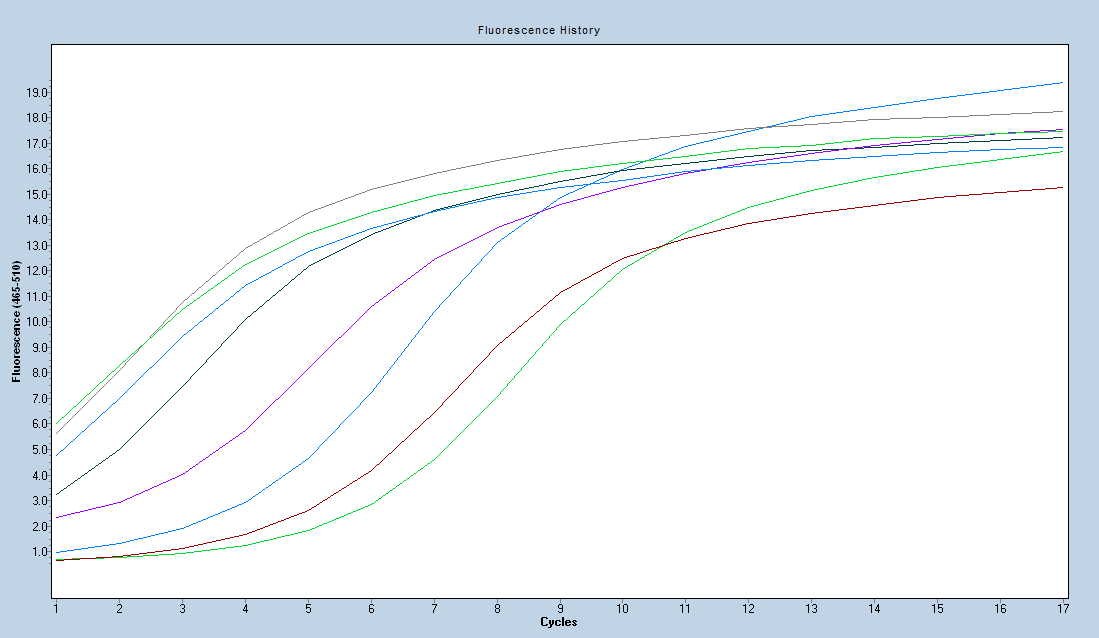
\includegraphics[scale=0.1]{qPCR_B}
%%     \caption{A}
%%     \label{fig:qpcr_a}
%%   \end{subfigure}
%%   \begin{subfigure}[htpb]{0.3\textwidth}
%%     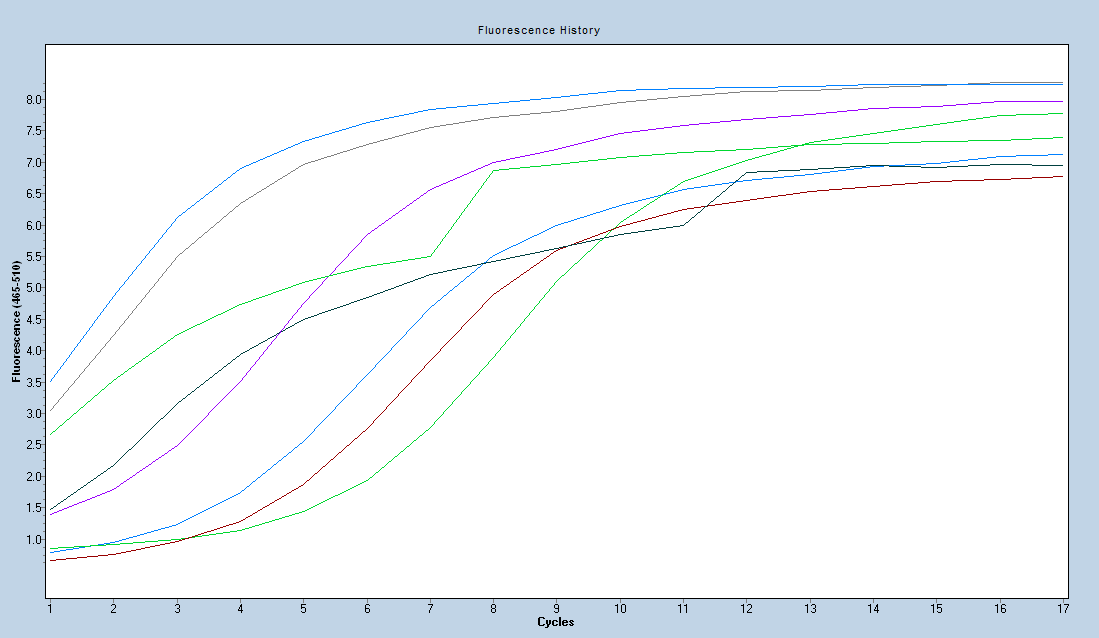
\includegraphics[scale=0.1]{qPCR_D}
%%     \caption{B}
%%     \label{fig:qpcr_b}
%%   \end{subfigure}
%%   \begin{subfigure}[htpb]{0.3\textwidth}
%%     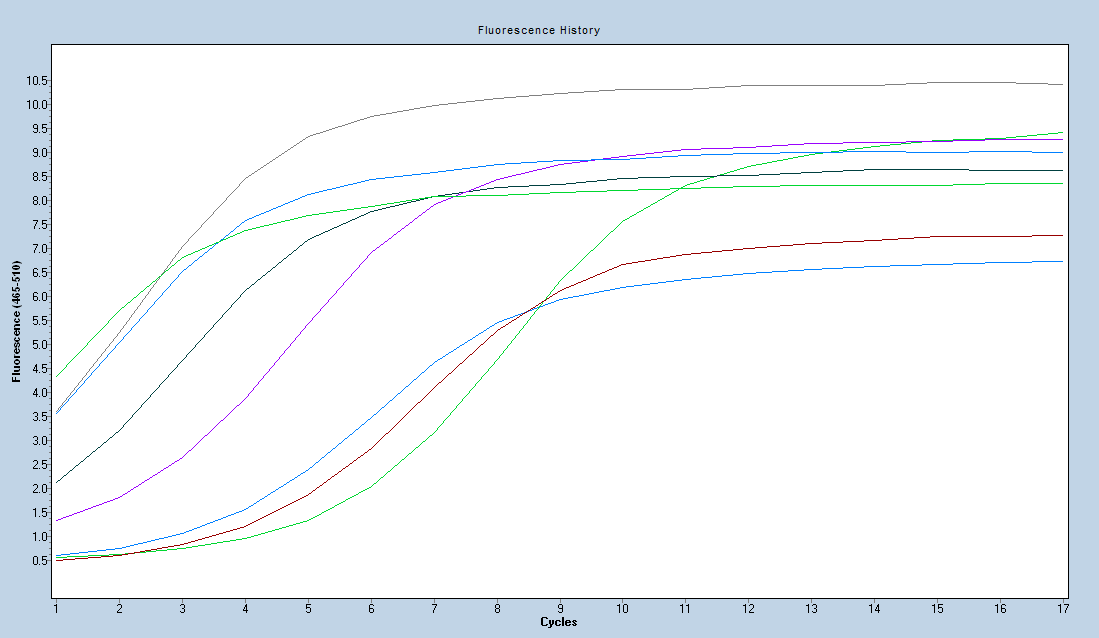
\includegraphics[scale=0.1]{qPCR_F}
%%     \caption{C}
%%     \label{fig:qpcr_c}
%%   \end{subfigure}
%%   \caption{A - row B, B - row D, C - row H}
%%   \label{fig:qpcr}
%% \end{figure}

\chapter{PCR Bias}
\label{ch:pcrbias}

\section{Introduction}
\label{sec:pcrbias_intro}

\subsection{Origin of PCR bias}
\label{ssec:pcrbias_intro_origin}

PCR is a known source of bias in massively parallel sequencing \citep{olova_comparison_2018}.  Among the processes in Illumina sequencing, PCR amplification during library preparation has been identified as the major source of bias.
% The corresponding figure from Aird et al. would be useful here
\citet{aird_analyzing_2011} measured frequencies of amplicons of varying GC content after each step in library preparation for Illumina sequencing, and found that DNA shearing, adapter ligation, gel size selection did not significantly introduce biases in response to GC content.  However, PCR depleted loci with GC content exceeding 65\% to the order of 1\% of the reference loci with intermediate GC content, and it also depleted loci with GC content lower than 12\% to the order of 10\% of the reference loci.  This pattern was observed even for 10 PCR cycles.

% == Not relevant to project ==
%Furthermore, amplification-free sequencing methods exhibited less bias than methods that rely on sequencing.  The amplification-free Pacific Biosciences sequencing introduced the least bias, followed by Illumina and Ion Torrent sequencing \citep{ross_characterizing_2013}. All methods exhibited biases for extremely low and extremely high GC content as described by \citet{aird_analyzing_2011}, but combining data from two sequencing technologies has been shown to potentially reduce bias.  However, amplification-free sequencing requires higher amounts of input DNA and more complicated experimental operations compared to sequencing methods that require amplification.

There are methods to mitigate this bias.  \citet{aird_analyzing_2011} found that this bias can be reduced by slowing the temperature ramping speed of thermocyclers, extending denaturation steps, and adding \SI{2}{\Molar} betaine.

Additionally, the choice of DNA polymerase enzyme has an effect.  Phusion DNA polymerase is commonly used because it has higher processivity and fidelity than most polymerases \citep{quail_optimal_2012}. Trying to reduce PCR bias by adding betaine and prolonging the denaturation step leads to a loss of high-AT sequences.  \citet{aird_analyzing_2011} also showed that replacing Phusion with AccuPrime Taq HiFi polymerase improved PCR bias.  Extension at \SI{60}{\celsius} using this enzyme retained more low-GC sequences, but also led to a decrease in yield of GC-rich reads.  \citet{quail_optimal_2012} showed that replacing Phusion with Kapa HiFi led to a more uniformm genome coverage.  However, this also led to a higher error rate, especially in TA-rich regions that Phusion often fails to amplify.

\subsection{How PCR bias affects reliability of sequencing results}
\label{ssec:pcrbias_intro_effects}

Commonly-used model organisms have GC content within the range in which bias is least likely introduced.  \emph{E. coli} and humans have genomes that have moderate GC content, with \emph{E. coli} having a GC content of 51\%.  PCR bias is still significant for these model organisms as they have important sequences that may be affected by PCR bias.  This includes single-nucleotide polymorphisms (SNPs), and GC-rich sequences like transcription start sites and first exons in eukaryotes.  %Additionally, humans exhibit `bad promoters'. % expand on the `bad promoters' data set from Ross et al.  Where did they get them, and what is their importance?

\subsection{Purpose of study}
\label{ssec:pcrbias_intro_why}

% QUESTION: evidence? is this actually true? ask fangjie
Although it is well-characterised that PCR introduces sequence biases, it is unknown which process within procedures that employ PCR amplification contributes the most to this bias, and to which degree.  Specifically, the biases introduced from the number of PCR cycles and from purification have not been characterised.  Such characterisation would be beneficial in developing a model to quantify PCR bias.  With such a model, these PCR biases can be removed in genomic studies to reveal true signals introduced by the factors tested in the relevant experiments.  PCR bias is especially relevant for nucleosome EMSA-SELEX employed in this project.  Sequence affinities for the nucleosome is weak, making the signal enrichment in the sequencing library weak, and makes it difficult to separate true signals introduced by nucleosome binding from biases introduced by PCR.  Both sequences bound to nucleosomes and sequences that are not exhibit the same PCR-introduced bias, rather than have biases that separate these two groups.

Here I assesed the sequence biases that could be introduced to the initial input library for nucleosome EMSA-SELEX.  I tested sequence biases introduced by the choice of DNA polymerase, choice of reagents, cycles of PCR, and purification of DNA after PCR.  From the resulting sequencing data, I assessed the distribution of k-mer nucleotides.  The experimental data led to constructing a model to account for PCR bias from these sources.

\section{Materials and Methods}
\label{sec:pcrbias_methods}

\subsection{DNA ligand design and preparation}
\label{ssec:pcrbias_methods_lig}

The same input library as \ref{ssec:emsaselex_methods_lig} was used, without methylation.

\subsection{Biases from enzymes}
\label{ssec:pcrbias_methods_enz}

PCR amplification followed manufacturers' specification for the following DNA polymerases: Phire Hot Start II DNA polymerase (ThermoFisher, F122S), Q5 Hot Start High-Fidelity DNA polymerase (New England BioLabs, M0493S), DreamTaq Hot Start DNA Polymerase (ThermoFisher, EP1701), and Phusion High-Fidelity DNA Polymerase (ThermoFisher, F530L).

For each enzyme, the input library was diluted by factors and then amplified for numbers of cycles as specified:

\begin{itemize}
  \item Dilute by a factor of $2^{4}$, then amplify for 8 cycles
  \item Dilute by a factor of $2^{8}$, then amplify for 12 cycles
  \item Dilute by a factor of $2^{12}$, then amplify for 16 cycles
  \item Dilute by a factor of $2^{16}$, then amplify for 20 cycles
  \item Dilute by a factor of $2^{20}$, then amplify for 24 cycles
\end{itemize}
    
To investigate bottleneck effects, the product from 24-cycle amplification was diluted by a factor of $2^{20}$.  From this, three samples were taken to be amplified using 24 cycles.

\subsection{Biases from PCR cycles}
\label{ssec:pcrbias_methods_pcr}

lig147 was diluted by a factor of $2^{20}$.  PCR amplification followed manufacturer's specification for Phusion High-Fidelity DNA Polymerase (ThermoFisher, F530L).  DNA was amplified for 4, 8, 12, 16, 20, 24, and 28 cycles, then re-diluted so that theoretical concentrations matched DNA that was amplified for 4 cycles.

\subsection{Biases from purification}
\label{ssec:pcrbias_methods_pur}

lig147 was purified using 1.2x Ampure beads (Agen Court AMPure) according to manufacturer's protocols, but with a \SI{15}{\micro\litre} elution volume.  Purification was repeated for 1, 2, 4, and 8 times.

\subsection{Biases from reagent vendors}
\label{ssec:pcrbias_methods_reagent}

lig147 was diluted by a factor of $2^{20}$.  It was then amplified for 24 cycles using manufacturer's specification for PCR amplification using Phusion High-Fidelity DNA Polymerase (ThermoFisher, F530L) and the reagents supplied by this vendor.

Combinations of Phusion High-Fidelity DNA Polymerase and dNTPs were investigated.  The polymerases used were from ThermoFisher (F530L) and New England BioLabs (M0530L).  The dNTPs used were from ThermoFisher (R0192), Agilent Technologies (200415-51), Kapa Biosystems (KN1009), and dNTPs containing 5-methylcytosine in place of dCTP from Zymo Research (D1030).  Twenty-four cycles of PCR using the eight combinations of polymerases and dNTPs proceeded according to manufacturer's specification for Phusion High-Fidelity DNA Polymerase (ThermoFisher, F530L).

\subsection{Sequencing}
\label{ssec:pcrbias_methods_seq}

The same procedures for sequencing as \ref{ssec:emsaselex_methods_seq} were used.

\subsection{Data analysis}
\label{ssec:pcrbias_methods_anal}

The same methods for fast Fourier transform and k-mer plot generation as \ref{ssec:emsaselex_methods_anal} were used.
% I can see this moved to results very easily
To investigate the effect of different vendors, a linear regression model was constructed.  The model used the frequencies of each nucleotide in the amplified library as the response variable.  The input variables were the enzyme vendor and dNTP vendor.

\section{Results}
\label{sec:pcrbias_results}

The initial input library lig147 was amplified and processed, with conditions varied to test biases introduced by polymerase enzymes, DNA purification, and reagent vendors.  After the PCR products were sequenced, the frequencies of each possible continuous 9-mer of nucleotides was counted.

% ORIGINAL
%% - Different oligonucleotide bias of different PCR enzymes
%% - The variance caused by bottleneck effect 
%% - Dependency of bias on PCR template concentration
%% - Bias caused by reagents from different company
%% - Bias from PCR Purification

\subsection{Biases from enzymes}
\label{ssec:pcrbias_result_enz}

\begin{figure}[htpb]
  \centering
  \begin{subfigure}[htpb]{0.5\textwidth}
    \centering
    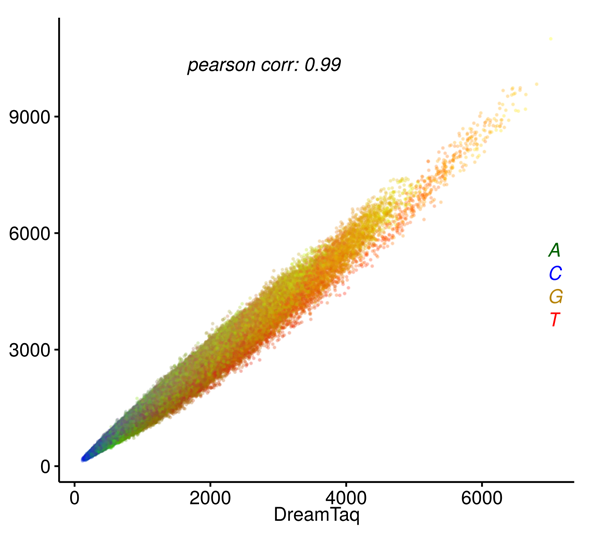
\includegraphics[width=0.5\textwidth]{kmer_dreamtaq}
    \caption{DreamTaq}
    \label{fig:kmer_enz_dreamtaq}
  \end{subfigure}
  \begin{subfigure}[htpb]{0.5\textwidth}
    \centering
    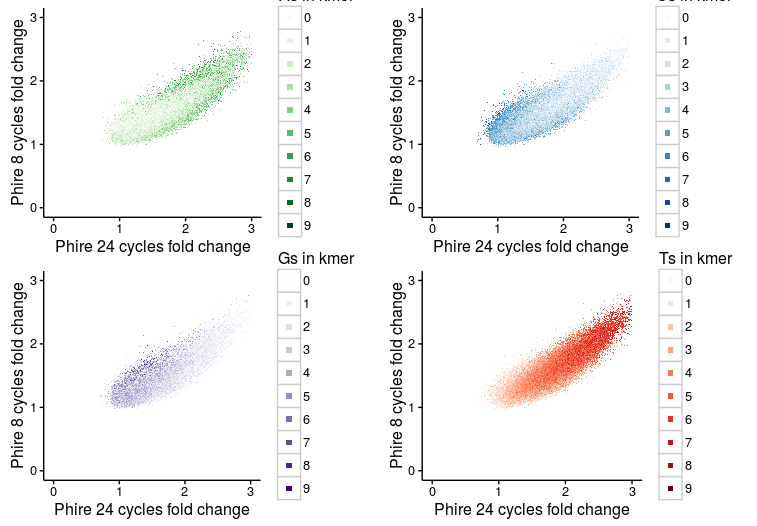
\includegraphics[width=0.5\textwidth]{kmer_phire}
    \caption{Phire}
    \label{fig:kmer_enz_phire}
  \end{subfigure}
  \begin{subfigure}[htpb]{0.5\textwidth}
    \centering
    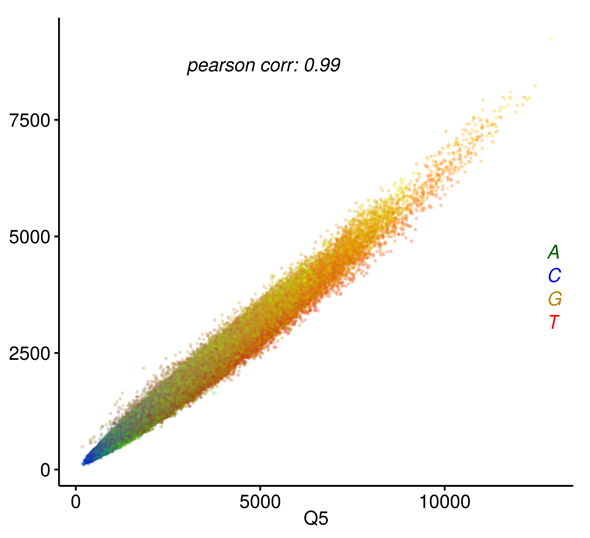
\includegraphics[width=0.5\textwidth]{kmer_q5}
    \caption{Q5}
    \label{fig:kmer_enz_q5}
  \end{subfigure}
  \begin{subfigure}[htpb]{0.5\textwidth}
    \centering
    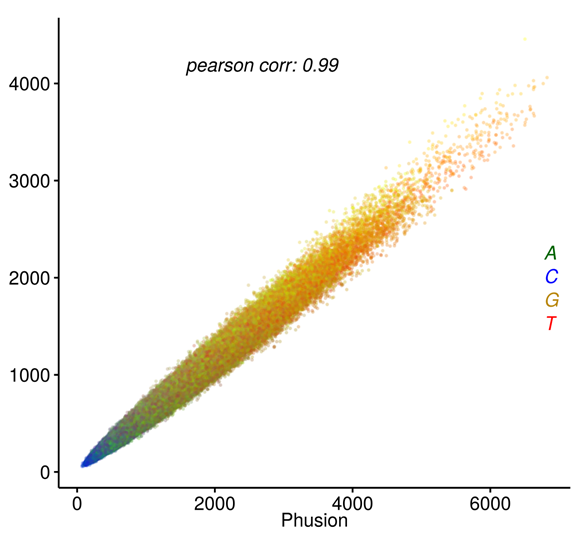
\includegraphics[width=0.5\textwidth]{kmer_phusion}
    \caption{Phusion}
    \label{fig:kmer_enz_phusion}
  \end{subfigure}
  \caption{9-mer count scatter plots showing the effect of polymerase enzyme.  Horizontal axes correspond to libraries after 24 cycles of PCR, while vertical axes correspond to libraries after 8 cycles of PCR.  Green indicates 9-mers consisting of predominantly adenines, blue cytosines, yellow guanines, and red thymines.}
  \label{fig:kmer_enz}
\end{figure}

Libraries amplified by Phusion, Phire, Dreamtaq, and Q5 DNA polymerase enzymes were analysed.  For each enzyme, the library from 24 cycles of PCR was compared to the library from 8 cycles of PCR (figure~\ref{fig:kmer_enz}).  All enzymes exhibited biases towards A and T, with Phusion exhibiting the weakest bias and Phire exhibiting the strongest bias.

% It seems that the plots don't work nicely.  I think it's most appropriate to move this to the discussion.  In the meantime, I might as well describe stuff here before I move them to the appropriate section.
\subsection{Biases from PCR cycles}
\label{ssec:pcrbias_result_pcr}

%% if decide to add figures, do it here

% Libraries resulting from using Phusion to amplify the lig147 input library over 8, 12, 16, 20, and 24 PCR cycles were analysed.  For each number of cycles, the correspond library was compared to the input library.  The results were very variable.  A possible explanation would be the instability of the adaptor addition step to prepare the ligands for sequencing: the adaptor addition step involves many cycles of PCR.  Additionally, the results also suggest that there is a lack of complexity of the library.  This lack of complexity increases the chance that sequences hybridise among each other, applying a selection bias on the library, and making the sequence biases more severe as a result.  To rectify these issues, a better input library should be constructed, with better filtering to remove sequences that have a tendency of causing primer dimers.

\subsection{Biases from purification}
\label{ssec:pcrbias_result_pur}

\begin{figure}[htpb]
  \centering
  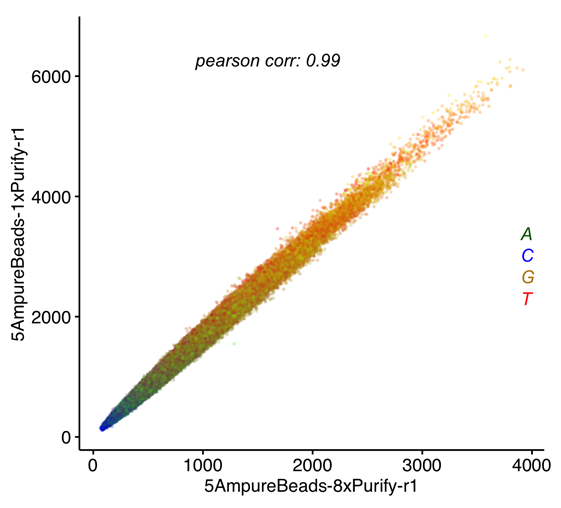
\includegraphics[width=0.7\textwidth]{kmer_ampure}
  \caption{9-mer count scatter plot showing the effect of AMPure bead purification.  The horizontal axis corresponds to the library after eight rounds of purification, while the vertical axis corresponds to the library after one round of purification.  Green indicates 9-mers consisting of predominantly adenines, blue cytosines, yellow guanines, and red thymines.}
  \label{fig:kmer_pur}
\end{figure}

Eight rounds of purification of the lig147 input library by AMPure beads did not introduce measurable nucleotide biases (figure~\ref{fig:kmer_pur}).  However, results from four rounds of purification (data not shown) seemed to suggest biases, but this bias is likely from the adaptor addition process. % QUESTION: how did we come to this conclusion?

\subsection{Biases from reagent vendors}
\label{ssec:pcrbias_result_reagent}

% I'm seriously considering changing these plots to dot plots and the vertical axes to be uniform around 0.20 to 0.30.  I have the data, not the code...
\begin{figure}[htpb]
  \centering
  \begin{subfigure}[htpb]{0.5\textwidth}
    \centering
    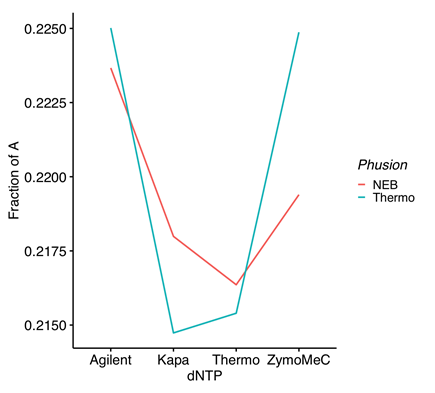
\includegraphics[width=0.5\textwidth]{linearmodel_a}
    \caption{adenine (A)}
    \label{fig:linearmodel_a}
  \end{subfigure}
  \begin{subfigure}[htpb]{0.5\textwidth}
    \centering
    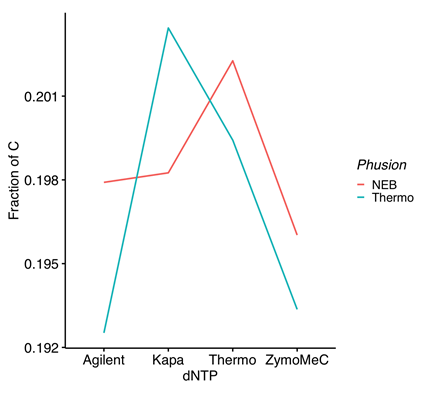
\includegraphics[width=0.5\textwidth]{linearmodel_c}
    \caption{cytosine (C)}
    \label{fig:linearmodel_c}
  \end{subfigure}
  \begin{subfigure}[htpb]{0.5\textwidth}
    \centering
    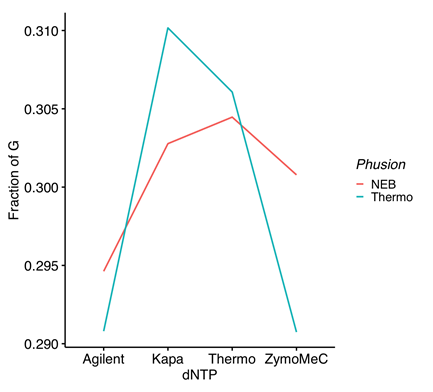
\includegraphics[width=0.5\textwidth]{linearmodel_g}
    \caption{guanine (G)}
    \label{fig:linearmodel_g}
  \end{subfigure}
  \begin{subfigure}[htpb]{0.5\textwidth}
    \centering
    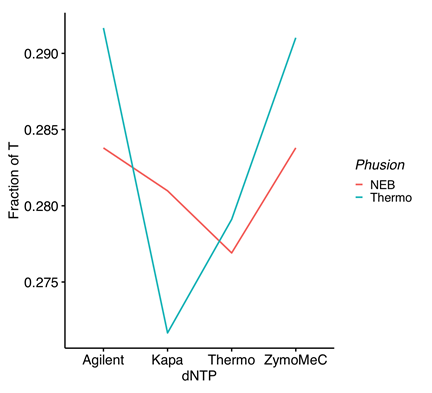
\includegraphics[width=0.5\textwidth]{linearmodel_t}
    \caption{thymine (T)}
    \label{fig:linearmodel_t}
  \end{subfigure}
  \caption{Fraction of each nucleotide after 24 cycles of amplification by each combination of dNTP and Phusion High-Fidelity DNA polymerase vendors.}
  \label{fig:linearmodel_nt}
\end{figure}

\begin{equation}
  \label{eqn:linearmodel}
  \textrm{fraction of nucleotide} \sim\ a (\textrm{enzyme vendor}) + b (\textrm{dNTP vendor}) + c
\end{equation}

\begin{table}[htpb]
  \centering
  \begin{tabular}{r}
     \\
    Phusion NEB\\
    dNTP Kapa\\
    dNTP Agilent\\
    dNTP ZymoMeC\\
  \end{tabular}%
  \pgfplotstabletypeset[
  col sep = comma,
  ]{linearmodel.csv}  
  \caption{Coefficients for the linear model to describe the contributions of dNTP and Phusion High-Fidelity DNA polymerase vendors to nucleotide fractions}
  \label{tab:linearmodel_coeffs}
\end{table}

% analyse the data and add how well the correlation is
\begin{figure}[htpb]
  \centering
  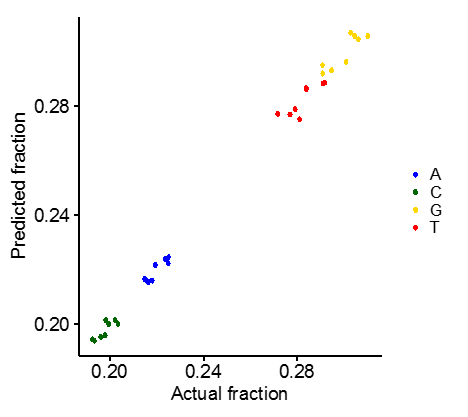
\includegraphics[width=\textwidth]{linearmodel_plot}
  \caption{Verification of linear model. R = 0.9XX}
  \label{fig:linearmodel_ver}
\end{figure}

Different combinations of vendors for dNTPs and Phusion High-Fidelity DNA polymerases for PCR were investigated.  The fractions of each nucleotide after 24 rounds of amplification were calculated for each combination (figure~\ref{fig:linearmodel_nt}).  These fractions were then used to construct a linear model (equation~\ref{eqn:linearmodel}) to describe the effects of dNTP and Phusion High-Fidelity DNA polymerase vendor on the fraction of the nucleotides. The model was then verified with experimental data (figure~\ref{fig:linearmodel_ver}).

\section{Discussion}
\label{sec:pcrbias_discussion}
%% - Relevance of such bias to previous sequencing data
%% - Hints to data analysis in the future 
%% - A few discussions about Troubleshooting

\chapter{Acknowledgements}
\label{ch:ack}

Acknowledgements.

\printbibliography

\end{document}
